\documentclass[a4paper,10pt]{article}
\usepackage{amsmath}
\usepackage{amssymb}
\usepackage[polish]{babel}
\usepackage{polski}
\usepackage[utf8]{inputenc}
\usepackage{indentfirst}
\usepackage{geometry}
\usepackage{array}
\usepackage[pdftex]{color,graphicx}
\usepackage{subfigure}
\usepackage{afterpage}
\usepackage{setspace}
\usepackage{color}
\usepackage{wrapfig}
\usepackage{listings}
\usepackage{datetime}

\renewcommand{\onehalfspacing}{\setstretch{1.6}}

\geometry{tmargin=2.5cm,bmargin=2.5cm,lmargin=2.5cm,rmargin=2.5cm}
\setlength{\parindent}{1cm}
\setlength{\parskip}{0mm}

\newenvironment{lista}{
\begin{itemize}
  \setlength{\itemsep}{1pt}
  \setlength{\parskip}{0pt}
  \setlength{\parsep}{0pt}
}{\end{itemize}}

\newcommand{\linia}{\rule{\linewidth}{0.4mm}}

\definecolor{lbcolor}{rgb}{0.95,0.95,0.95}
\lstset{
    backgroundcolor=\color{lbcolor},
    tabsize=4,
  language=C++,
  captionpos=b,
  tabsize=3,
  frame=lines,
  numbers=left,
  numberstyle=\tiny,
  numbersep=5pt,
  breaklines=true,
  showstringspaces=false,
  basicstyle=\footnotesize,
  identifierstyle=\color{magenta},
  keywordstyle=\color[rgb]{0,0,1},
  commentstyle=\color{Darkgreen},
  stringstyle=\color{red}
  }

\begin{document}

\noindent
\begin{tabular}{|c|p{11cm}|c|} \hline 
Z2 & Przemysław Kleszcz, Krzysztof Tatar & \ddmmyyyydate\today \tabularnewline
\hline 
\end{tabular}


\section*{Zadanie 2 - Rozmycie Gaussa w MPI}

Celem zadania było napisanie programu, który rozmywa zadane zdjęcie za pomocą algorytmu Gaussa z maską o wymiarach 5x5. Do poprawnego działania programu należy podać trzy argumenty wejściowe. Są to \emph{n -liczba procesów}, \emph{input\_image - ścieżka do pliku obrazu w formacie JPEG} i \emph{output\_image - ścieżka do pliku wyjściowego obrazu w formacie JPEG
}.Poniżej przedstawiony jest rysunek zastosowanej maski 5 x 5 wraz z wagami, które są wykorzystywane podczas przeprowadzania obliczeń.

\begin{figure}[!ht]
	\centering
 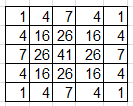
\includegraphics[width=0.2\textwidth]{3.png}
  \caption{Wykorzystana maska Gaussowska}
\end{figure}

Poniżej zaprezentowano główną funkcję programu odpowiedzialną za zrównoleglanie obliczeń oraz instrukcje MPI.

\begin{lstlisting}
    MPI_Send(dane, rozmiar, typ, destination, tag, communicator);
    MPI_Recv(data, size, type, destination, tag, communicator, MPI_STATUS_IGNORE);
Mat gauss(Mat picture, Mat pictureNew, int kernel[][5], int weight) {
	int y, x;
	int r, g, b;
	int i_x, i_y;
	for (y = 2; y < picture.rows - 2; y++)
	{
		for (x = 2; x < picture.cols - 2; x++)
		{
		...
		...
		...
		}
	}
	return pictureNew;
}
	MPI_Init(argc, argv);
	communicator = MPI_COMM_WORLD;
	MPI_Comm_rank(communicator, numberOfProcess);
	MPI_Comm_size(communicator, processes);
	MPI_Finalize();
\end{lstlisting}

W powyższym programie został zastosowany algorytm filtrowania za pomocą którego posiadamy możliwość rozmycia podanego obrazka. Każdy proces wykonuje rozmywanie niezależnie od własnej części obrazka. Poza wyliczeniem wartości piksela wynikowego, w każdym kroku należy sprawdzić czy nie znajdujemy się na brzegu obrazu i wtedy wykonać odpowiednią korektę.

Funkcje MPI użyte w programie.
\begin{lstlisting}
MPI_Init(argc, argv);
\end{lstlisting}
Funkcja inicjalizuje środowisko wykonywania programu, m.in. tworzy domyślny komunikator \newline MPI\_COMM\_WORLD. Dopiero od momentu wywołania MPI\_Init można używać pozostałych funkcji MPI
\begin{lstlisting}
MPI_Comm_rank(MPI_COMM_WORLD, numberOfProcess);
\end{lstlisting}
Funkcja pobiera numer aktualnego procesu (w obrębie komunikatora comm) i umieszcza go w zmiennej rank.
\begin{lstlisting}
MPI_Comm_size(MPI_COMM_WORLD, processes);
\end{lstlisting}
Funkcja pobiera ilość procesów (w obrębie komunikatora comm i umieszcza ją w zmiennej size.
\begin{lstlisting}
MPI_Finalize()
\end{lstlisting}
Funkcja zwalnia zasoby używane przez MPI i przygotowuje system do zamknięcia.

\begin{lstlisting}
MPI_Recv(data, size, type, destination, tag, communicator, MPI_STATUS_IGNORE);
\end{lstlisting}
Funkcja odczytuje z kolejki komunikatora communicator (z ewentualnym blokowaniem do czasu nadejścia) pierwszy komunikat od procesu source oznaczony znacznikiem tag typu datatype. Wynik umieszczany jest w buforze data a status operacji w zmiennej status.

\begin{lstlisting}
 MPI_Send(dane, rozmiar, typ, destination, tag, communicator);
\end{lstlisting}
Funkcja wysyła komunikat typu datatype do procesu numer dest oznaczony znacznikiem tag w obrębie komunikatora communicator.
Typ komunikatu jest zawarty w zmiennej datatype i może to być którymś z predefiniowanych typów np.  MPI\_INT lub inne. Tag jest liczbą w zakresie [0..MPI\_TAG\_UB] i określa dodatkowy typ komunikatu wykorzystywany przy selektywnym odbiorze funkcją MPI\_Recv.

\begin{figure}[!ht]
	\centering
 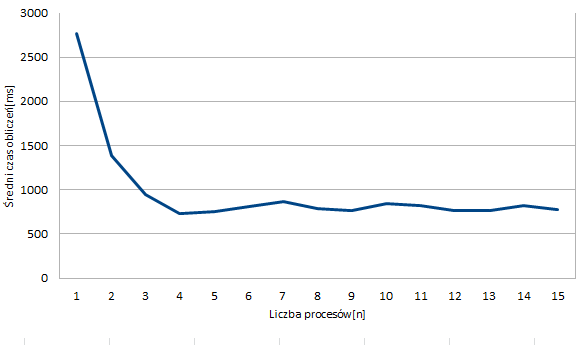
\includegraphics[width=0.7\textwidth]{1.png}
  \caption{Wykres średniego czasu obliczeń}
\end{figure}

Z powyższego rysunku można wywnioskować, że średni czas obliczeń dynamicznie malał dla pierwszych 4 procesów. Następnie dla kolejnych procesów średni czas przyjmuje postać sinusoidy.
Poniższy rysunek jest dobrym przykładem opisanego zjawiska.

\begin{figure}[ht]
	\centering
  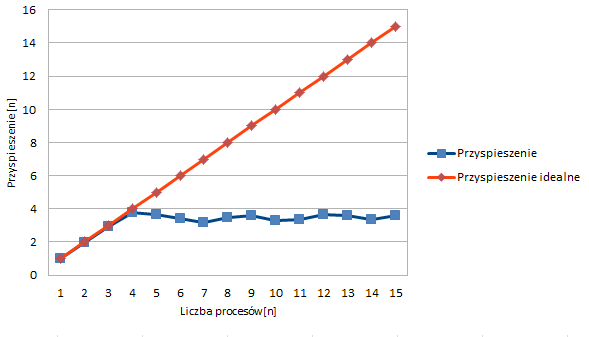
\includegraphics[width=0.7\textwidth]{2.png}
  \caption{Wykres przyspieszenia}
\end{figure}

Powyższe zadanie zostało zrównoleglone dzięki bibliotece MPI (Message Passing Interface). Udało się uzyskać czterokrotne przyspieszenie dla 4 procesów. Dla kolejnych 11 procesów, w tym przykładzie nie wpłynęły znacząco na wydajność, wykres ma postać sinusoidy.


\end{document}
